\documentclass[]{article}
\usepackage{lmodern}
\usepackage{amssymb,amsmath}
\usepackage{ifxetex,ifluatex}
\usepackage{fixltx2e} % provides \textsubscript
\ifnum 0\ifxetex 1\fi\ifluatex 1\fi=0 % if pdftex
  \usepackage[T1]{fontenc}
  \usepackage[utf8]{inputenc}
\else % if luatex or xelatex
  \ifxetex
    \usepackage{mathspec}
  \else
    \usepackage{fontspec}
  \fi
  \defaultfontfeatures{Ligatures=TeX,Scale=MatchLowercase}
\fi
% use upquote if available, for straight quotes in verbatim environments
\IfFileExists{upquote.sty}{\usepackage{upquote}}{}
% use microtype if available
\IfFileExists{microtype.sty}{%
\usepackage{microtype}
\UseMicrotypeSet[protrusion]{basicmath} % disable protrusion for tt fonts
}{}
\usepackage[margin=1in]{geometry}
\usepackage{hyperref}
\hypersetup{unicode=true,
            pdftitle={Final project: Statistical Inference},
            pdfauthor={Kwatanwa17},
            pdfborder={0 0 0},
            breaklinks=true}
\urlstyle{same}  % don't use monospace font for urls
\usepackage{color}
\usepackage{fancyvrb}
\newcommand{\VerbBar}{|}
\newcommand{\VERB}{\Verb[commandchars=\\\{\}]}
\DefineVerbatimEnvironment{Highlighting}{Verbatim}{commandchars=\\\{\}}
% Add ',fontsize=\small' for more characters per line
\usepackage{framed}
\definecolor{shadecolor}{RGB}{248,248,248}
\newenvironment{Shaded}{\begin{snugshade}}{\end{snugshade}}
\newcommand{\KeywordTok}[1]{\textcolor[rgb]{0.13,0.29,0.53}{\textbf{#1}}}
\newcommand{\DataTypeTok}[1]{\textcolor[rgb]{0.13,0.29,0.53}{#1}}
\newcommand{\DecValTok}[1]{\textcolor[rgb]{0.00,0.00,0.81}{#1}}
\newcommand{\BaseNTok}[1]{\textcolor[rgb]{0.00,0.00,0.81}{#1}}
\newcommand{\FloatTok}[1]{\textcolor[rgb]{0.00,0.00,0.81}{#1}}
\newcommand{\ConstantTok}[1]{\textcolor[rgb]{0.00,0.00,0.00}{#1}}
\newcommand{\CharTok}[1]{\textcolor[rgb]{0.31,0.60,0.02}{#1}}
\newcommand{\SpecialCharTok}[1]{\textcolor[rgb]{0.00,0.00,0.00}{#1}}
\newcommand{\StringTok}[1]{\textcolor[rgb]{0.31,0.60,0.02}{#1}}
\newcommand{\VerbatimStringTok}[1]{\textcolor[rgb]{0.31,0.60,0.02}{#1}}
\newcommand{\SpecialStringTok}[1]{\textcolor[rgb]{0.31,0.60,0.02}{#1}}
\newcommand{\ImportTok}[1]{#1}
\newcommand{\CommentTok}[1]{\textcolor[rgb]{0.56,0.35,0.01}{\textit{#1}}}
\newcommand{\DocumentationTok}[1]{\textcolor[rgb]{0.56,0.35,0.01}{\textbf{\textit{#1}}}}
\newcommand{\AnnotationTok}[1]{\textcolor[rgb]{0.56,0.35,0.01}{\textbf{\textit{#1}}}}
\newcommand{\CommentVarTok}[1]{\textcolor[rgb]{0.56,0.35,0.01}{\textbf{\textit{#1}}}}
\newcommand{\OtherTok}[1]{\textcolor[rgb]{0.56,0.35,0.01}{#1}}
\newcommand{\FunctionTok}[1]{\textcolor[rgb]{0.00,0.00,0.00}{#1}}
\newcommand{\VariableTok}[1]{\textcolor[rgb]{0.00,0.00,0.00}{#1}}
\newcommand{\ControlFlowTok}[1]{\textcolor[rgb]{0.13,0.29,0.53}{\textbf{#1}}}
\newcommand{\OperatorTok}[1]{\textcolor[rgb]{0.81,0.36,0.00}{\textbf{#1}}}
\newcommand{\BuiltInTok}[1]{#1}
\newcommand{\ExtensionTok}[1]{#1}
\newcommand{\PreprocessorTok}[1]{\textcolor[rgb]{0.56,0.35,0.01}{\textit{#1}}}
\newcommand{\AttributeTok}[1]{\textcolor[rgb]{0.77,0.63,0.00}{#1}}
\newcommand{\RegionMarkerTok}[1]{#1}
\newcommand{\InformationTok}[1]{\textcolor[rgb]{0.56,0.35,0.01}{\textbf{\textit{#1}}}}
\newcommand{\WarningTok}[1]{\textcolor[rgb]{0.56,0.35,0.01}{\textbf{\textit{#1}}}}
\newcommand{\AlertTok}[1]{\textcolor[rgb]{0.94,0.16,0.16}{#1}}
\newcommand{\ErrorTok}[1]{\textcolor[rgb]{0.64,0.00,0.00}{\textbf{#1}}}
\newcommand{\NormalTok}[1]{#1}
\usepackage{graphicx,grffile}
\makeatletter
\def\maxwidth{\ifdim\Gin@nat@width>\linewidth\linewidth\else\Gin@nat@width\fi}
\def\maxheight{\ifdim\Gin@nat@height>\textheight\textheight\else\Gin@nat@height\fi}
\makeatother
% Scale images if necessary, so that they will not overflow the page
% margins by default, and it is still possible to overwrite the defaults
% using explicit options in \includegraphics[width, height, ...]{}
\setkeys{Gin}{width=\maxwidth,height=\maxheight,keepaspectratio}
\IfFileExists{parskip.sty}{%
\usepackage{parskip}
}{% else
\setlength{\parindent}{0pt}
\setlength{\parskip}{6pt plus 2pt minus 1pt}
}
\setlength{\emergencystretch}{3em}  % prevent overfull lines
\providecommand{\tightlist}{%
  \setlength{\itemsep}{0pt}\setlength{\parskip}{0pt}}
\setcounter{secnumdepth}{0}
% Redefines (sub)paragraphs to behave more like sections
\ifx\paragraph\undefined\else
\let\oldparagraph\paragraph
\renewcommand{\paragraph}[1]{\oldparagraph{#1}\mbox{}}
\fi
\ifx\subparagraph\undefined\else
\let\oldsubparagraph\subparagraph
\renewcommand{\subparagraph}[1]{\oldsubparagraph{#1}\mbox{}}
\fi

%%% Use protect on footnotes to avoid problems with footnotes in titles
\let\rmarkdownfootnote\footnote%
\def\footnote{\protect\rmarkdownfootnote}

%%% Change title format to be more compact
\usepackage{titling}

% Create subtitle command for use in maketitle
\newcommand{\subtitle}[1]{
  \posttitle{
    \begin{center}\large#1\end{center}
    }
}

\setlength{\droptitle}{-2em}

  \title{Final project: Statistical Inference}
    \pretitle{\vspace{\droptitle}\centering\huge}
  \posttitle{\par}
    \author{Kwatanwa17}
    \preauthor{\centering\large\emph}
  \postauthor{\par}
      \predate{\centering\large\emph}
  \postdate{\par}
    \date{4/9/2018}


\begin{document}
\maketitle

\subsection{Overview}\label{overview}

This report consists of two parts. The first part corresponds to the
comparison of the simulation sample mean to the theorical mean of
exponential distribution. In the second part, we conducted t test using
ToothGroth data set.

\subsection{Part 1: Simulation
Exercise}\label{part-1-simulation-exercise}

\subsubsection{Simulation}\label{simulation}

We simulated 1000 times 40 samples of exponential distribution with
lambda = 40 and averaged it by each simulation. Likewise, we took 40
samples from the theorical distribution 1000 times.

Note that the mean of exponential distribution is 1/lambda and its
standard deviation is also 1/lambda. So, in our case, the mean and
standard deviation is 1/0.2 = 5.

\begin{Shaded}
\begin{Highlighting}[]
\NormalTok{n <-}\StringTok{ }\DecValTok{40}
\NormalTok{lambda <-}\StringTok{ }\FloatTok{0.2}
\NormalTok{nosim <-}\StringTok{ }\DecValTok{1000}

\KeywordTok{set.seed}\NormalTok{(}\DecValTok{1}\NormalTok{)}
\NormalTok{Simulation <-}\StringTok{ }\KeywordTok{replicate}\NormalTok{(nosim, }\KeywordTok{rexp}\NormalTok{(n, lambda))}
\NormalTok{Simulation_means <-}\StringTok{ }\KeywordTok{apply}\NormalTok{(Simulation, }\DecValTok{2}\NormalTok{, mean)}
\NormalTok{Simulation_vars <-}\StringTok{ }\KeywordTok{apply}\NormalTok{(Simulation, }\DecValTok{2}\NormalTok{, var)}

\KeywordTok{set.seed}\NormalTok{(}\DecValTok{1}\NormalTok{)}
\NormalTok{Theorical <-}\StringTok{ }\KeywordTok{replicate}\NormalTok{(nosim, }\KeywordTok{rnorm}\NormalTok{(}\DecValTok{40}\NormalTok{, }\DataTypeTok{mean =} \DecValTok{1}\OperatorTok{/}\FloatTok{0.2}\NormalTok{, }\DataTypeTok{sd =} \DecValTok{1}\OperatorTok{/}\FloatTok{0.2}\NormalTok{))}
\NormalTok{Theorical_means <-}\StringTok{ }\KeywordTok{apply}\NormalTok{(Theorical, }\DecValTok{2}\NormalTok{, mean)}
\NormalTok{Theorical_vars <-}\StringTok{ }\KeywordTok{apply}\NormalTok{(Theorical, }\DecValTok{2}\NormalTok{, var)}

\NormalTok{dat <-}\StringTok{ }\KeywordTok{data.frame}\NormalTok{(}
      \DataTypeTok{Mean =} \KeywordTok{c}\NormalTok{(Simulation_means, Theorical_means),}
      \DataTypeTok{Variance =} \KeywordTok{c}\NormalTok{(Simulation_vars, Theorical_vars),}
      \DataTypeTok{Type =} \KeywordTok{rep}\NormalTok{(}\KeywordTok{c}\NormalTok{(}\StringTok{"Simulation"}\NormalTok{, }\StringTok{"Theorical"}\NormalTok{), }\DataTypeTok{each =}\NormalTok{ nosim)}
\NormalTok{    )}
\end{Highlighting}
\end{Shaded}

\subsubsection{Sample Mean versus Theoretical
Mean}\label{sample-mean-versus-theoretical-mean}

Both distributions are very closed

\begin{Shaded}
\begin{Highlighting}[]
\KeywordTok{summary}\NormalTok{(Simulation_means)}
\end{Highlighting}
\end{Shaded}

\begin{verbatim}
##    Min. 1st Qu.  Median    Mean 3rd Qu.    Max. 
##   3.108   4.445   4.950   4.990   5.492   7.491
\end{verbatim}

\begin{Shaded}
\begin{Highlighting}[]
\KeywordTok{summary}\NormalTok{(Theorical_means)}
\end{Highlighting}
\end{Shaded}

\begin{verbatim}
##    Min. 1st Qu.  Median    Mean 3rd Qu.    Max. 
##   2.637   4.456   4.993   4.989   5.532   7.823
\end{verbatim}

\begin{Shaded}
\begin{Highlighting}[]
\KeywordTok{library}\NormalTok{(ggplot2)}
\NormalTok{g <-}\StringTok{ }\KeywordTok{ggplot}\NormalTok{(dat, }\KeywordTok{aes}\NormalTok{(}\DataTypeTok{x =}\NormalTok{ Mean, }\DataTypeTok{fill =}\NormalTok{ Type)) }\OperatorTok{+}
\StringTok{  }\KeywordTok{geom_histogram}\NormalTok{(}\DataTypeTok{binwidth =} \FloatTok{0.5}\NormalTok{, }\DataTypeTok{color =} \StringTok{"black"}\NormalTok{) }\OperatorTok{+}
\StringTok{  }\KeywordTok{facet_wrap}\NormalTok{(}\OperatorTok{~}\NormalTok{Type, }\DataTypeTok{ncol =} \DecValTok{2}\NormalTok{)}
\NormalTok{g}
\end{Highlighting}
\end{Shaded}

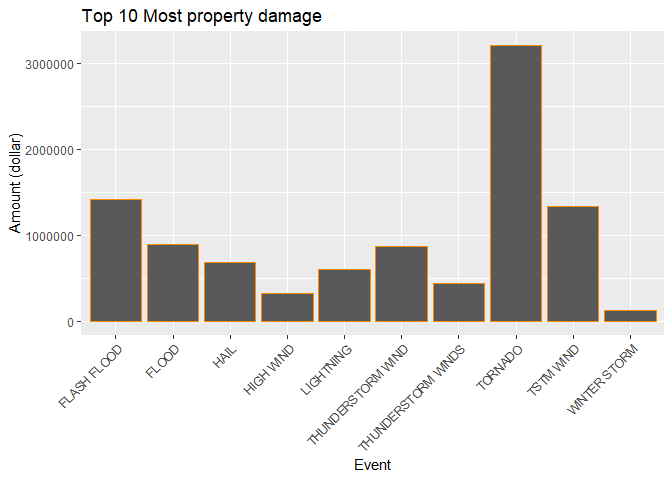
\includegraphics{CourseProject_files/figure-latex/unnamed-chunk-3-1.pdf}

\subsubsection{Sample Variance versus Theoretical
Variance}\label{sample-variance-versus-theoretical-variance}

The distribution of simulation variances are more skewed than the
theorical one.

\begin{Shaded}
\begin{Highlighting}[]
\KeywordTok{summary}\NormalTok{(Simulation_vars)}
\end{Highlighting}
\end{Shaded}

\begin{verbatim}
##    Min. 1st Qu.  Median    Mean 3rd Qu.    Max. 
##   6.153  16.912  22.739  25.065  30.465  99.828
\end{verbatim}

\begin{Shaded}
\begin{Highlighting}[]
\KeywordTok{summary}\NormalTok{(Theorical_vars)}
\end{Highlighting}
\end{Shaded}

\begin{verbatim}
##    Min. 1st Qu.  Median    Mean 3rd Qu.    Max. 
##   10.79   21.08   24.90   25.14   29.01   46.90
\end{verbatim}

\begin{Shaded}
\begin{Highlighting}[]
\NormalTok{g2 <-}\StringTok{ }\KeywordTok{ggplot}\NormalTok{(dat, }\KeywordTok{aes}\NormalTok{(}\DataTypeTok{x =}\NormalTok{ Variance, }\DataTypeTok{fill =}\NormalTok{ Type)) }\OperatorTok{+}
\StringTok{  }\KeywordTok{geom_histogram}\NormalTok{(}\DataTypeTok{binwidth =} \DecValTok{5}\NormalTok{,  }\DataTypeTok{color =} \StringTok{"black"}\NormalTok{) }\OperatorTok{+}
\StringTok{  }\KeywordTok{facet_wrap}\NormalTok{(}\OperatorTok{~}\NormalTok{Type, }\DataTypeTok{ncol =} \DecValTok{2}\NormalTok{)}
\NormalTok{g2}
\end{Highlighting}
\end{Shaded}

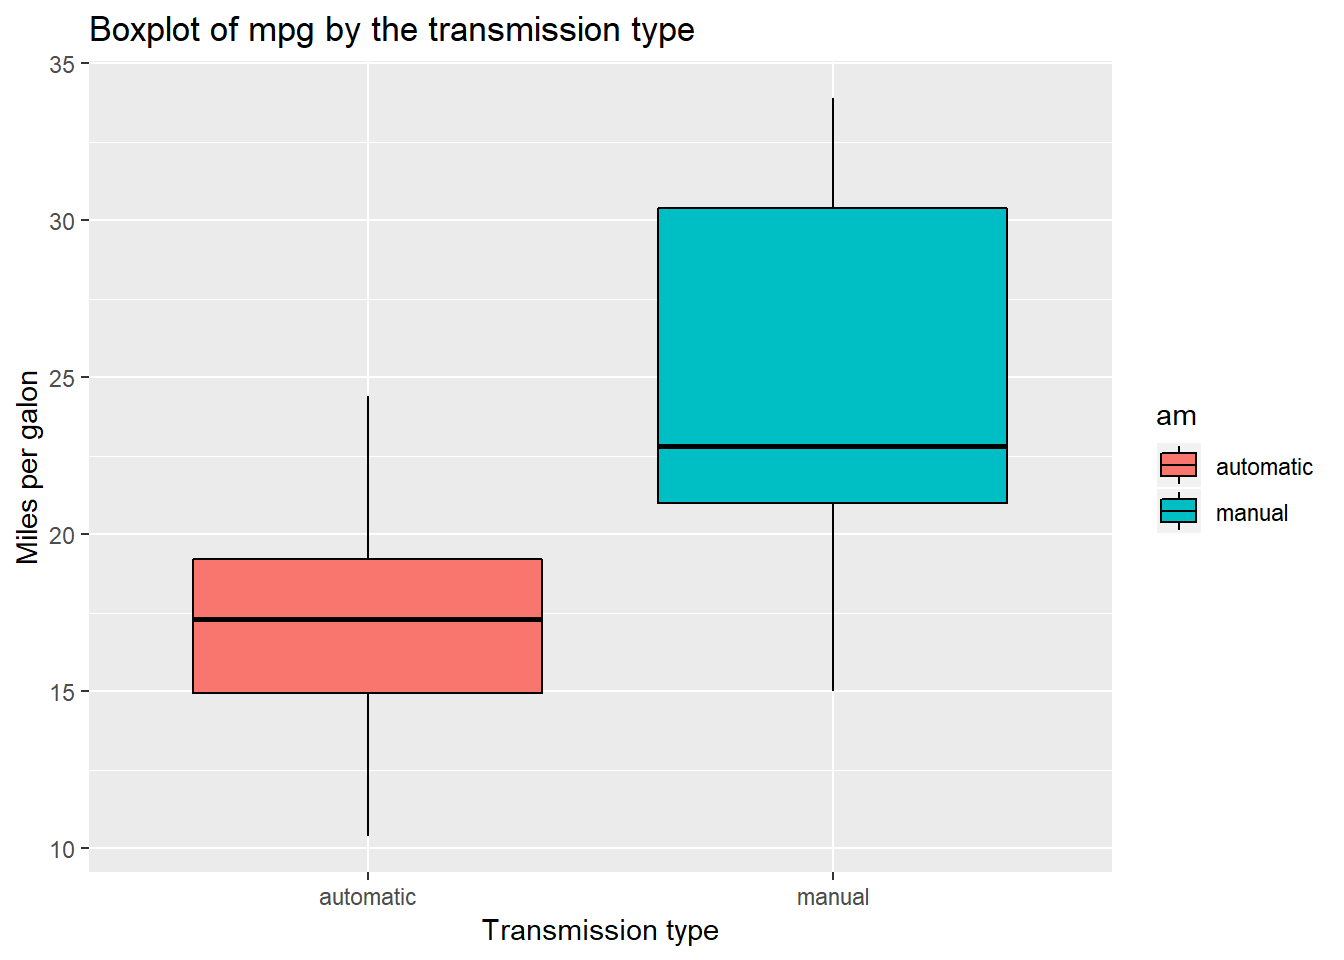
\includegraphics{CourseProject_files/figure-latex/unnamed-chunk-5-1.pdf}

\subsubsection{Approximately normal}\label{approximately-normal}

The red curve represents the density of normal distribution with the
mean and standard deviation of simulation means. Except the distribution
of simulation variances, all the distributions seem to be distributed
normally.

\begin{Shaded}
\begin{Highlighting}[]
\NormalTok{scaled_dat <-}\StringTok{ }\KeywordTok{as.data.frame}\NormalTok{(}\KeywordTok{apply}\NormalTok{(}
  \KeywordTok{data.frame}\NormalTok{(Simulation_means, Theorical_means, Simulation_vars, Theorical_vars), }
  \DecValTok{2}\NormalTok{, scale))}

\KeywordTok{library}\NormalTok{(tidyr)}
\NormalTok{scaled_dat_updated <-}\StringTok{ }\NormalTok{tidyr}\OperatorTok{::}\KeywordTok{gather}\NormalTok{(scaled_dat, }\DataTypeTok{key =}\NormalTok{ Distribution_type, }\DataTypeTok{value =}\NormalTok{ z_score)}

\NormalTok{g5 <-}\StringTok{ }\KeywordTok{ggplot}\NormalTok{(scaled_dat_updated, }\KeywordTok{aes}\NormalTok{(}\DataTypeTok{x =}\NormalTok{ z_score, }\DataTypeTok{fill =}\NormalTok{Distribution_type)) }\OperatorTok{+}
\StringTok{  }\KeywordTok{geom_histogram}\NormalTok{(}\KeywordTok{aes}\NormalTok{(}\DataTypeTok{y =}\NormalTok{ ..density..), }\DataTypeTok{color =} \StringTok{"black"}\NormalTok{) }\OperatorTok{+}
\StringTok{  }\KeywordTok{facet_wrap}\NormalTok{(}\OperatorTok{~}\NormalTok{Distribution_type, }\DataTypeTok{ncol =} \DecValTok{2}\NormalTok{, }\DataTypeTok{nrow =} \DecValTok{2}\NormalTok{) }\OperatorTok{+}
\StringTok{  }\KeywordTok{stat_function}\NormalTok{(}\DataTypeTok{fun =}\NormalTok{ dnorm, }\DataTypeTok{color =} \StringTok{"brown"}\NormalTok{, }\DataTypeTok{args =} \KeywordTok{list}\NormalTok{(}\DataTypeTok{mean =} \DecValTok{0}\NormalTok{))}
\NormalTok{g5}
\end{Highlighting}
\end{Shaded}

\begin{verbatim}
## `stat_bin()` using `bins = 30`. Pick better value with `binwidth`.
\end{verbatim}

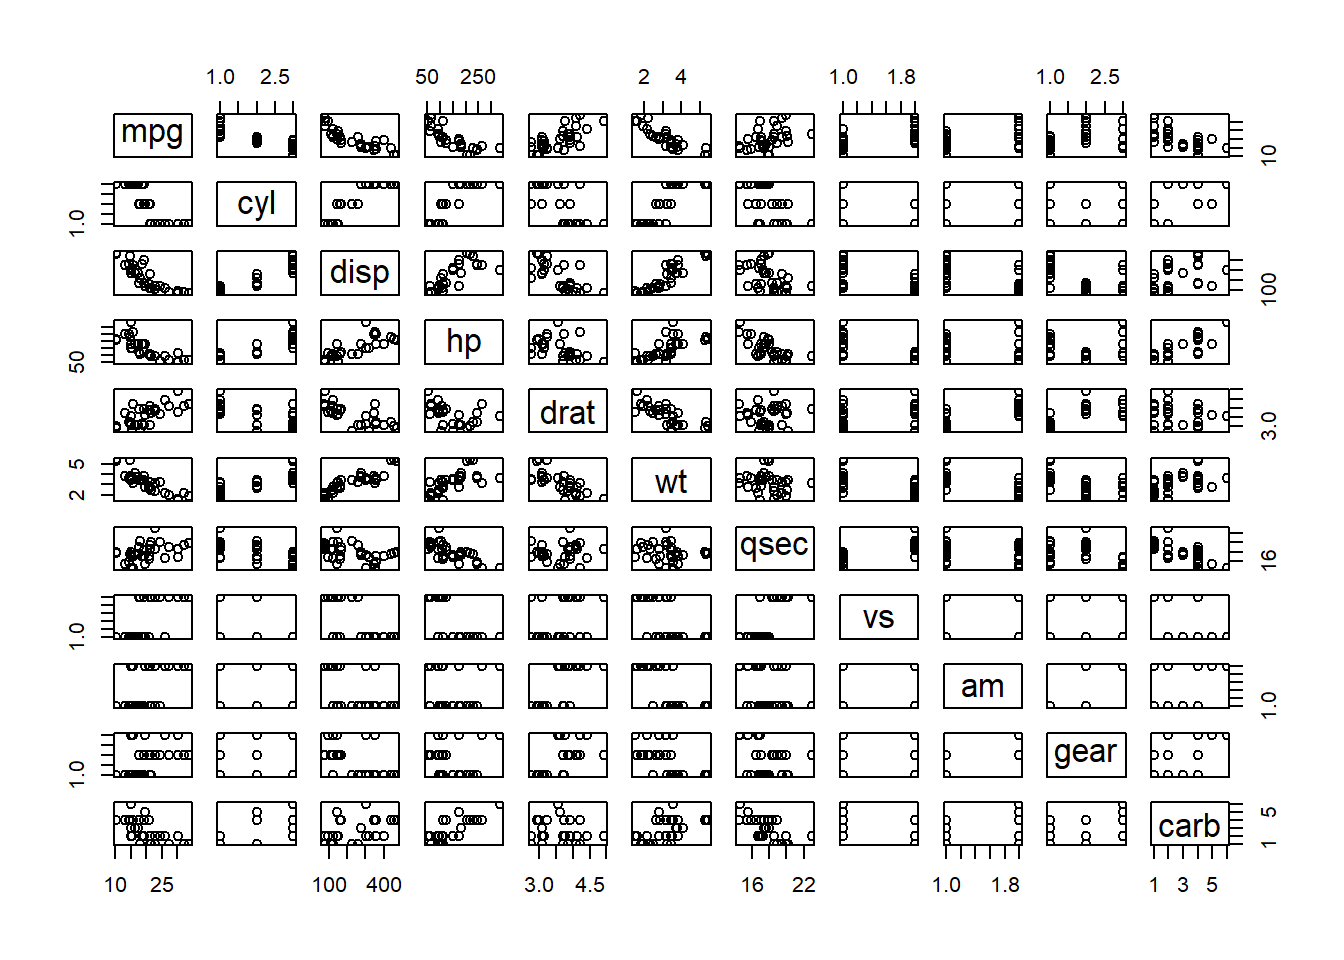
\includegraphics{CourseProject_files/figure-latex/unnamed-chunk-6-1.pdf}

\subsection{Part 2: Basic Inferential Data
Analysis}\label{part-2-basic-inferential-data-analysis}

Load the data set.

\begin{Shaded}
\begin{Highlighting}[]
\KeywordTok{library}\NormalTok{(datasets)}
\KeywordTok{data}\NormalTok{(}\StringTok{"ToothGrowth"}\NormalTok{)}
\end{Highlighting}
\end{Shaded}

\subsubsection{Summary of the data}\label{summary-of-the-data}

Notice that the variable dose is the quantity of dose which ranges from
0.5 to 2. There is the same number of subjects with respect to the supp
variable (OJ/VC).

\begin{Shaded}
\begin{Highlighting}[]
\KeywordTok{summary}\NormalTok{(ToothGrowth)}
\end{Highlighting}
\end{Shaded}

\begin{verbatim}
##       len        supp         dose      
##  Min.   : 4.20   OJ:30   Min.   :0.500  
##  1st Qu.:13.07   VC:30   1st Qu.:0.500  
##  Median :19.25           Median :1.000  
##  Mean   :18.81           Mean   :1.167  
##  3rd Qu.:25.27           3rd Qu.:2.000  
##  Max.   :33.90           Max.   :2.000
\end{verbatim}

\subsubsection{T test two sided test}\label{t-test-two-sided-test}

\begin{Shaded}
\begin{Highlighting}[]
\NormalTok{VC <-}\StringTok{ }\KeywordTok{subset}\NormalTok{(ToothGrowth, supp }\OperatorTok{==}\StringTok{ "VC"}\NormalTok{)}
\NormalTok{OJ <-}\StringTok{ }\KeywordTok{subset}\NormalTok{(ToothGrowth, supp }\OperatorTok{==}\StringTok{ "OJ"}\NormalTok{)}
\end{Highlighting}
\end{Shaded}

\begin{Shaded}
\begin{Highlighting}[]
\KeywordTok{t.test}\NormalTok{(VC}\OperatorTok{$}\NormalTok{dose, OJ}\OperatorTok{$}\NormalTok{dose, }\DataTypeTok{paired =} \OtherTok{FALSE}\NormalTok{, }\DataTypeTok{var.equal =} \OtherTok{FALSE}\NormalTok{)}
\end{Highlighting}
\end{Shaded}

\begin{verbatim}
## 
##  Welch Two Sample t-test
## 
## data:  VC$dose and OJ$dose
## t = 0, df = 58, p-value = 1
## alternative hypothesis: true difference in means is not equal to 0
## 95 percent confidence interval:
##  -0.3278171  0.3278171
## sample estimates:
## mean of x mean of y 
##  1.166667  1.166667
\end{verbatim}

\begin{Shaded}
\begin{Highlighting}[]
\KeywordTok{t.test}\NormalTok{(VC}\OperatorTok{$}\NormalTok{len, OJ}\OperatorTok{$}\NormalTok{len, }\DataTypeTok{paired =} \OtherTok{FALSE}\NormalTok{, }\DataTypeTok{var.equal =} \OtherTok{FALSE}\NormalTok{)}
\end{Highlighting}
\end{Shaded}

\begin{verbatim}
## 
##  Welch Two Sample t-test
## 
## data:  VC$len and OJ$len
## t = -1.9153, df = 55.309, p-value = 0.06063
## alternative hypothesis: true difference in means is not equal to 0
## 95 percent confidence interval:
##  -7.5710156  0.1710156
## sample estimates:
## mean of x mean of y 
##  16.96333  20.66333
\end{verbatim}

As a result of the analysis of the experiment data, there is no
diference of tooth length by the supplement type (orange juice vs
ascorbic acid). On the other hand, it is quite clear that there would
not be difference by levels of Vitamin C (variable dose).For more
information, please see R help page (``The Effect of Vitamin C on Tooth
Growth in Guinea Pigs'':
\url{http://www.is.titech.ac.jp/~mase/mase/html.jp/temp/ToothGrowth.jp.html}).


\end{document}
